% !TEX root = main.tex
\chapter{System overview}\label{cha:systemOverview}

This chapter provides the reader with a brief overview of the whole collimator system. This will be followed by a more detailed description of the rotational stage.

\section{Crystal collimators}
A collimator is a specially designed device, built to interfere with the beam and clean it from surrounding halo particles. To be able to meet the future demand of higher energy levels, a more efficient collmator is being devloped at CERN. This new collimator will utilze a crystaline solid to extract particles from the beam. The collimator consists of a T-shape structure containg two movable linear axes and one rotational stage. Each linear axis is driven by a stepping motor, labeled as \emph{M1} and \emph{M2} in Figure~\ref{fig:collimator-side}, seperately controlled in open-loop by an individual drive unit. The motor driving the vertical axis, \emph{M1}, is used to move a piece of beampipe down inside the T-shape, giving access to the horizontal axis, driven by \emph{M2}, to move the rotaional stage (including the crystal) into the beampipe to interfere with the beam. The directions of the crystal's linear and rotational movement are indicated by the arrows in Figure~\ref{fig:collimator-top}.
During operation, Physicists will drive the crystal close to the beam, enter it with an angle and rotate it slightly (in the range of \unit{10}{\milli\rad}) until the channeling effect is detected. Channeled particles will then be bent off the bem core and abosorbed further down the beam pipe.

 \begin{figure}[tpb]
   \centering %crop: left bottom right top
   \subfloat[][\label{fig:collimator-side}Collimator from side]{
   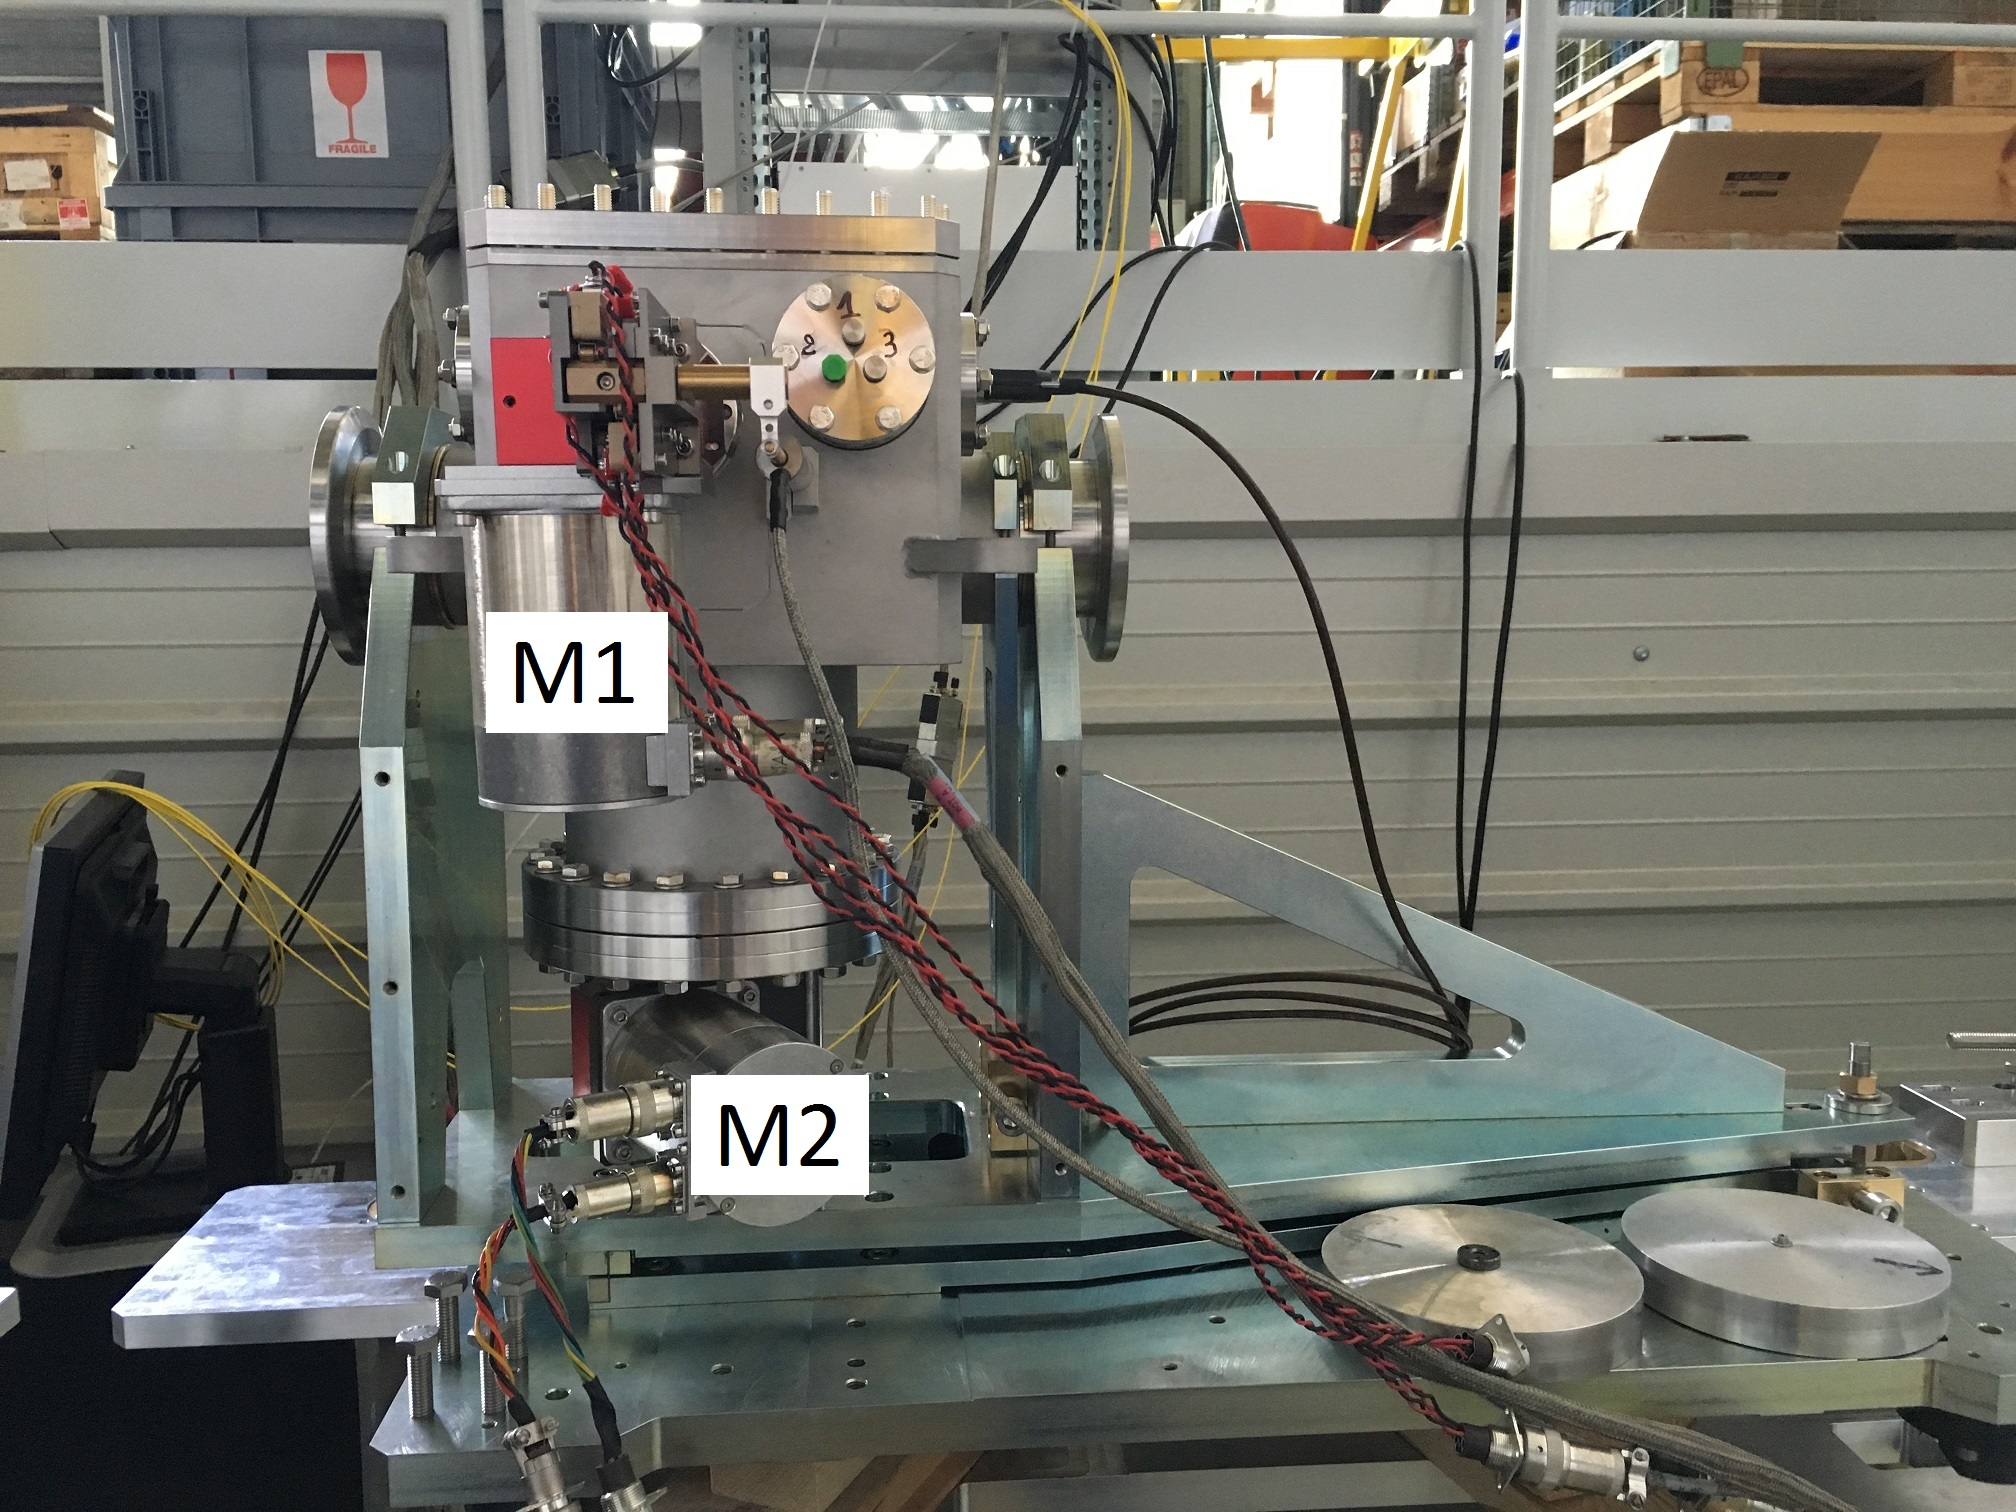
\includegraphics[width=0.5\textwidth, trim=10cm 12cm 50cm 7cm, clip=true]{fig/collimator-side}}
   \qquad
   \subfloat[][\label{fig:collimator-top}Collimator from top]{
   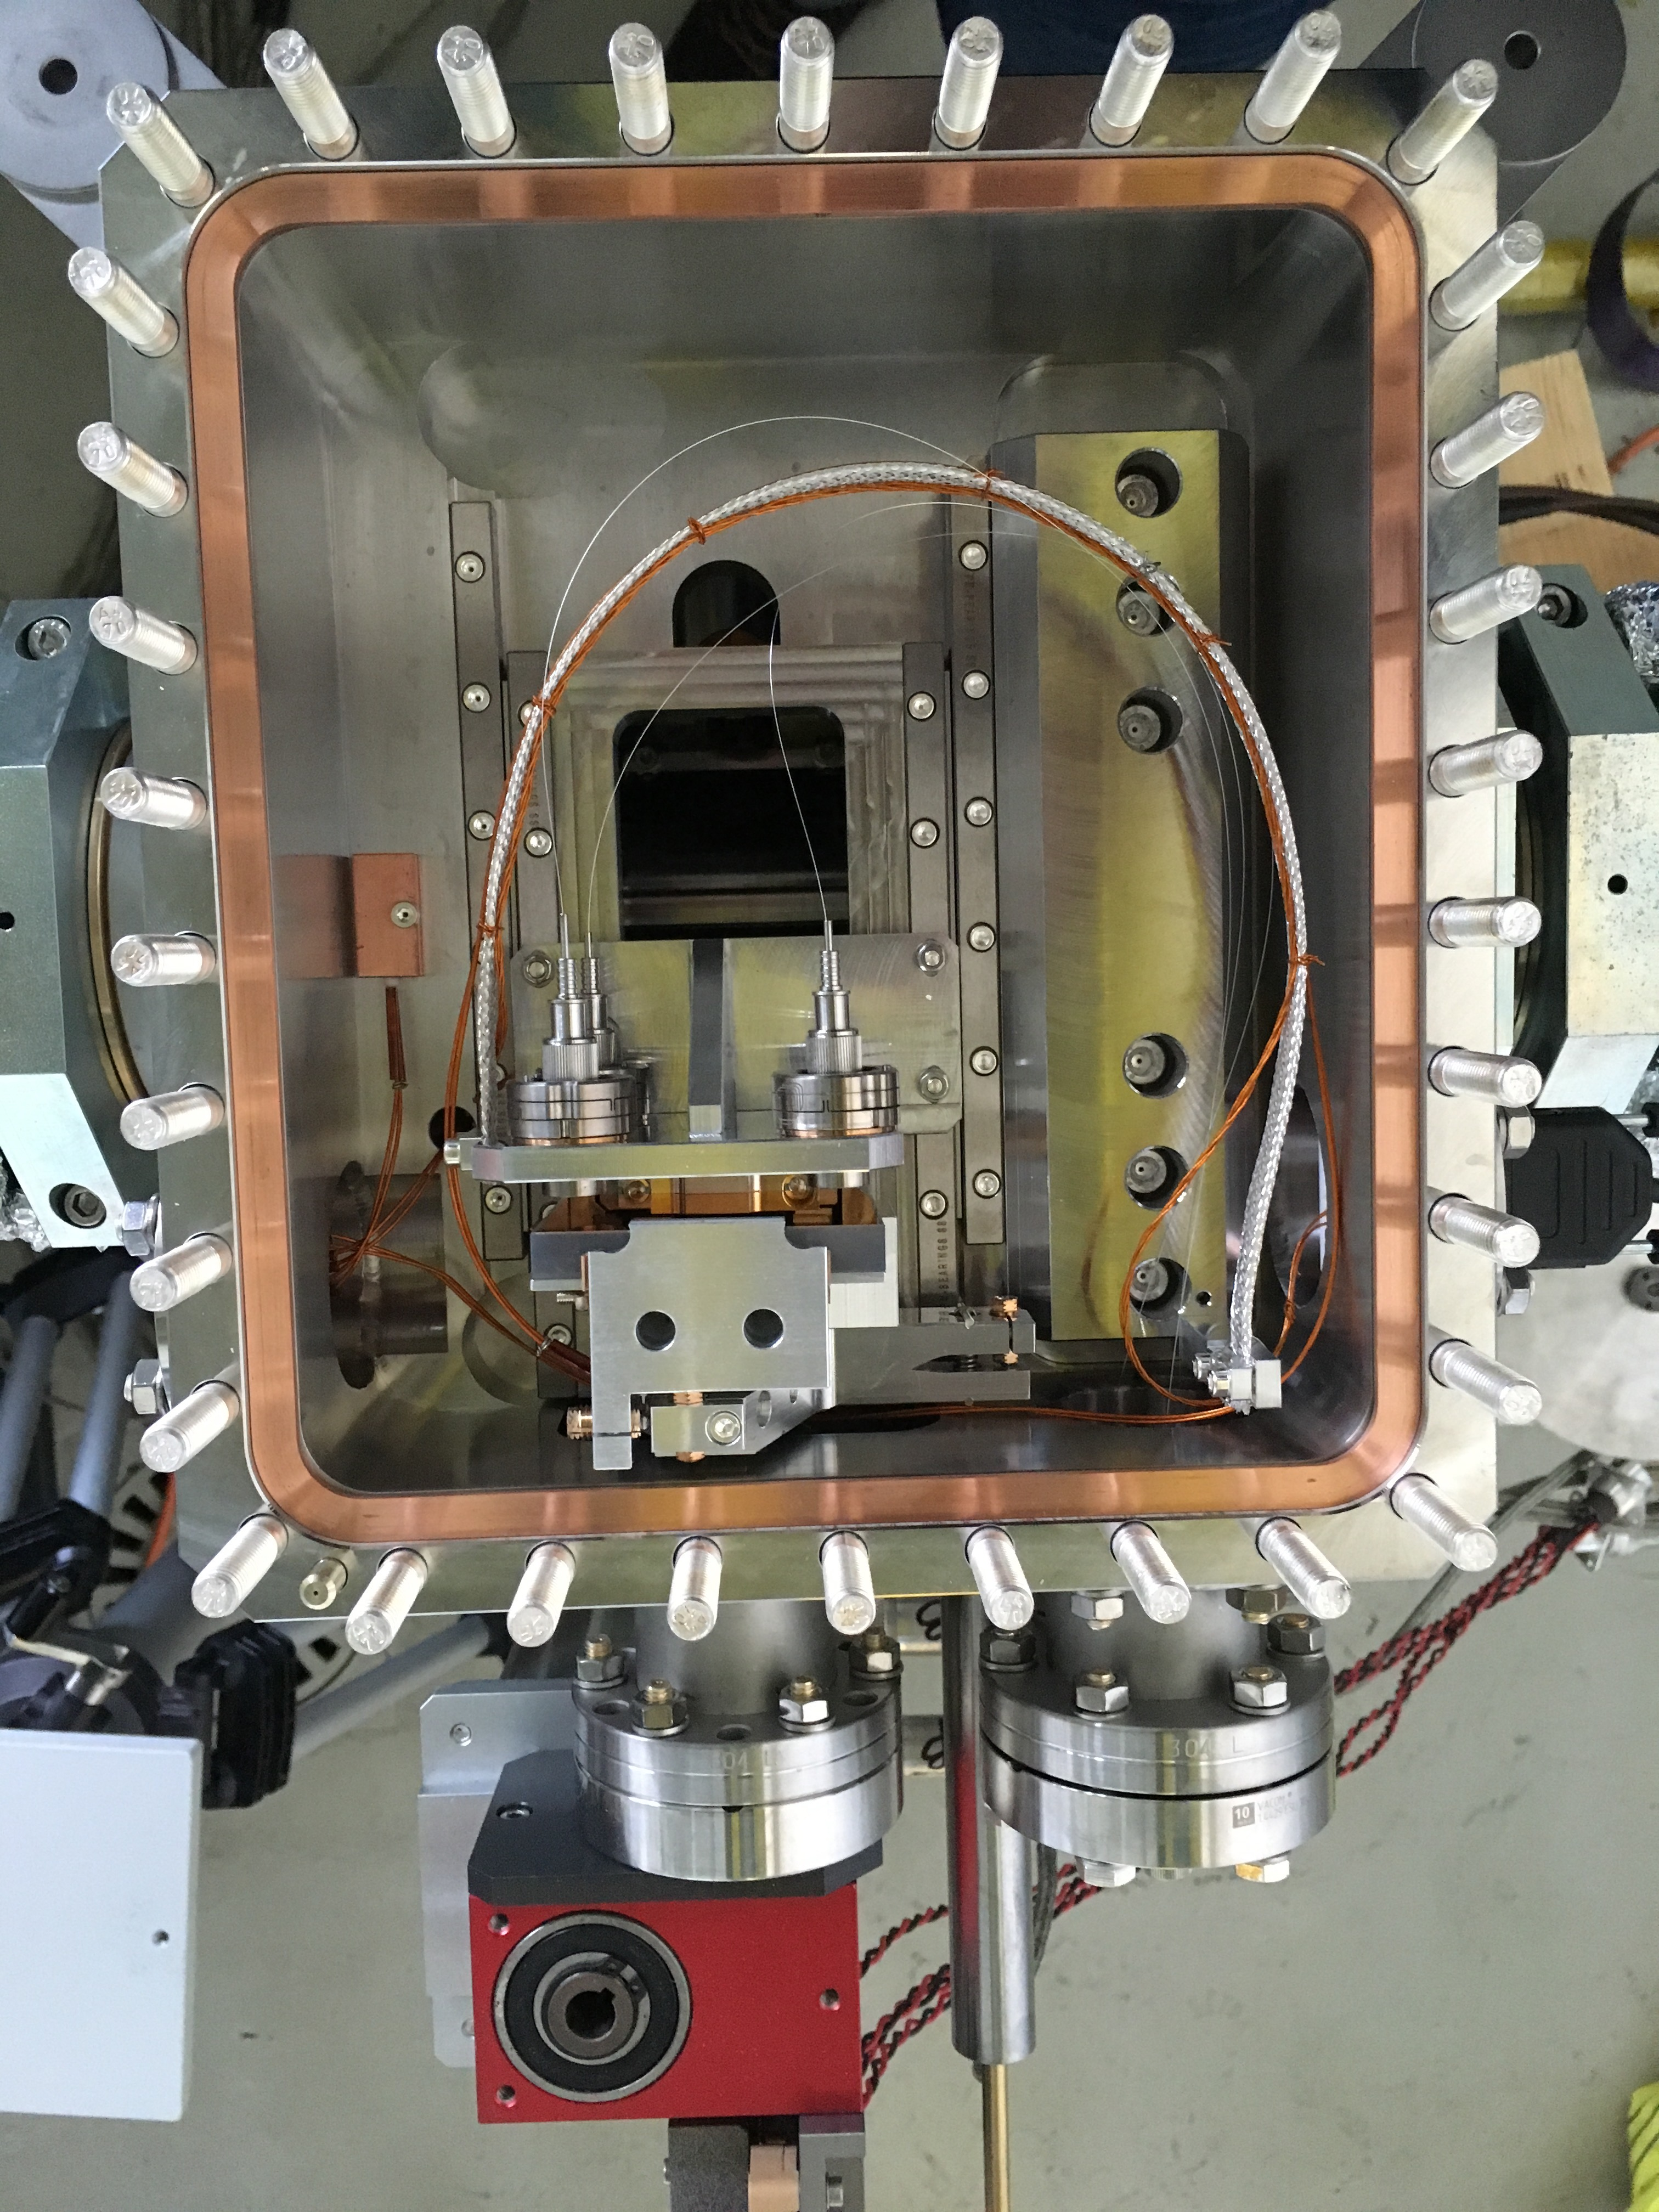
\includegraphics[width=0.4\textwidth, trim=0cm 0cm 0cm 0cm, clip=true]{fig/collimator-top}}
   \caption{\label{fig:collimator} Illustrates the collimator from the side (a) and the top (b).}
 \end{figure}

\section{Rotational stage}
The rotational stage as shown in Figure? is composed by a monolitic structure, a prestressed piezo stack actuator and an interferometer measurement system. The flexure-hinge based structure, avoids sliding parts and thereby enhance precision by reducing the number of nonlinear effects (e.g. backlash and friction). A prestressed piezo stack actuator is exploited to generate the rotaional movement by interacting on a point 4mm away from the center of rotation, see Figure. This amplyfing structure gives the rotational stage a range of \unit{20}{\milli\rad}. For the measurement system, 3 interferometric heads are placed as in Figure ?, pointing towards a mirror mounted ontop of to the rotaional head, perpendicular to the plane of rotation. The setup allows for measurements of both the yaw and roll angle (the coordnate system is defined with respect to the beam). The yaw angle is used as feedback to the rotational stage control loop. The spring, depicted in Figure?, prestresses the \abbrPESA in order to enhace the overall stiffness of the stage as well as keeping the stackplates in place (the stack is nonglued to be sufficient in a radioactive area). This combinataion leads to an unmistaken resonsant structure, due to the characteristics of the \abbrPESA demanding in combination with the spring, demanding a properly designed controller. The system moving the crystal, i.e. the linear axis driven by \emph{M2} and the rotaional stage needs to be able to track reference trajectories at ramp rates of \unit{100}{\micro\radianpersecond} and reject external disturbances to maintain a maximum tracking error of $\pm$\unit{1}{\micro\rad}.

\section{Piezoelectric stack actuator}
The rotaional stage uses a linear piezoelectric stack actuator to create the movement. It provides a displacement range from 0 to \unit{30}{\micro\meter}, corresponding to 0 and 150V, respectively.

\section{Nonlinear effects}

\section{System identification}
